\section{Architecture}
This section describes the software architecture proposed by this project in order to realize the Transparent scheduling model over heterogeneous devices and, consequently, satisfy the requirements and use cases previously described.

\textit{Figure \ref{fig:architecture_complete}} provides a complete view of the Architecture; being a complex project based on the interaction between multiple distributed entities, the schema will be divided in three areas (easier to understand) that will be discussed in the following sections:
\begin{itemize}
    \item Cloud Services area (\textit{section \ref{cloud_services_area}})
    \item Contributor area (\textit{section \ref{contributor_area}})
    \item Customer area (\textit{section \ref{customer_area}})
\end{itemize}
\begin{figure}[!ht]
    \centering
    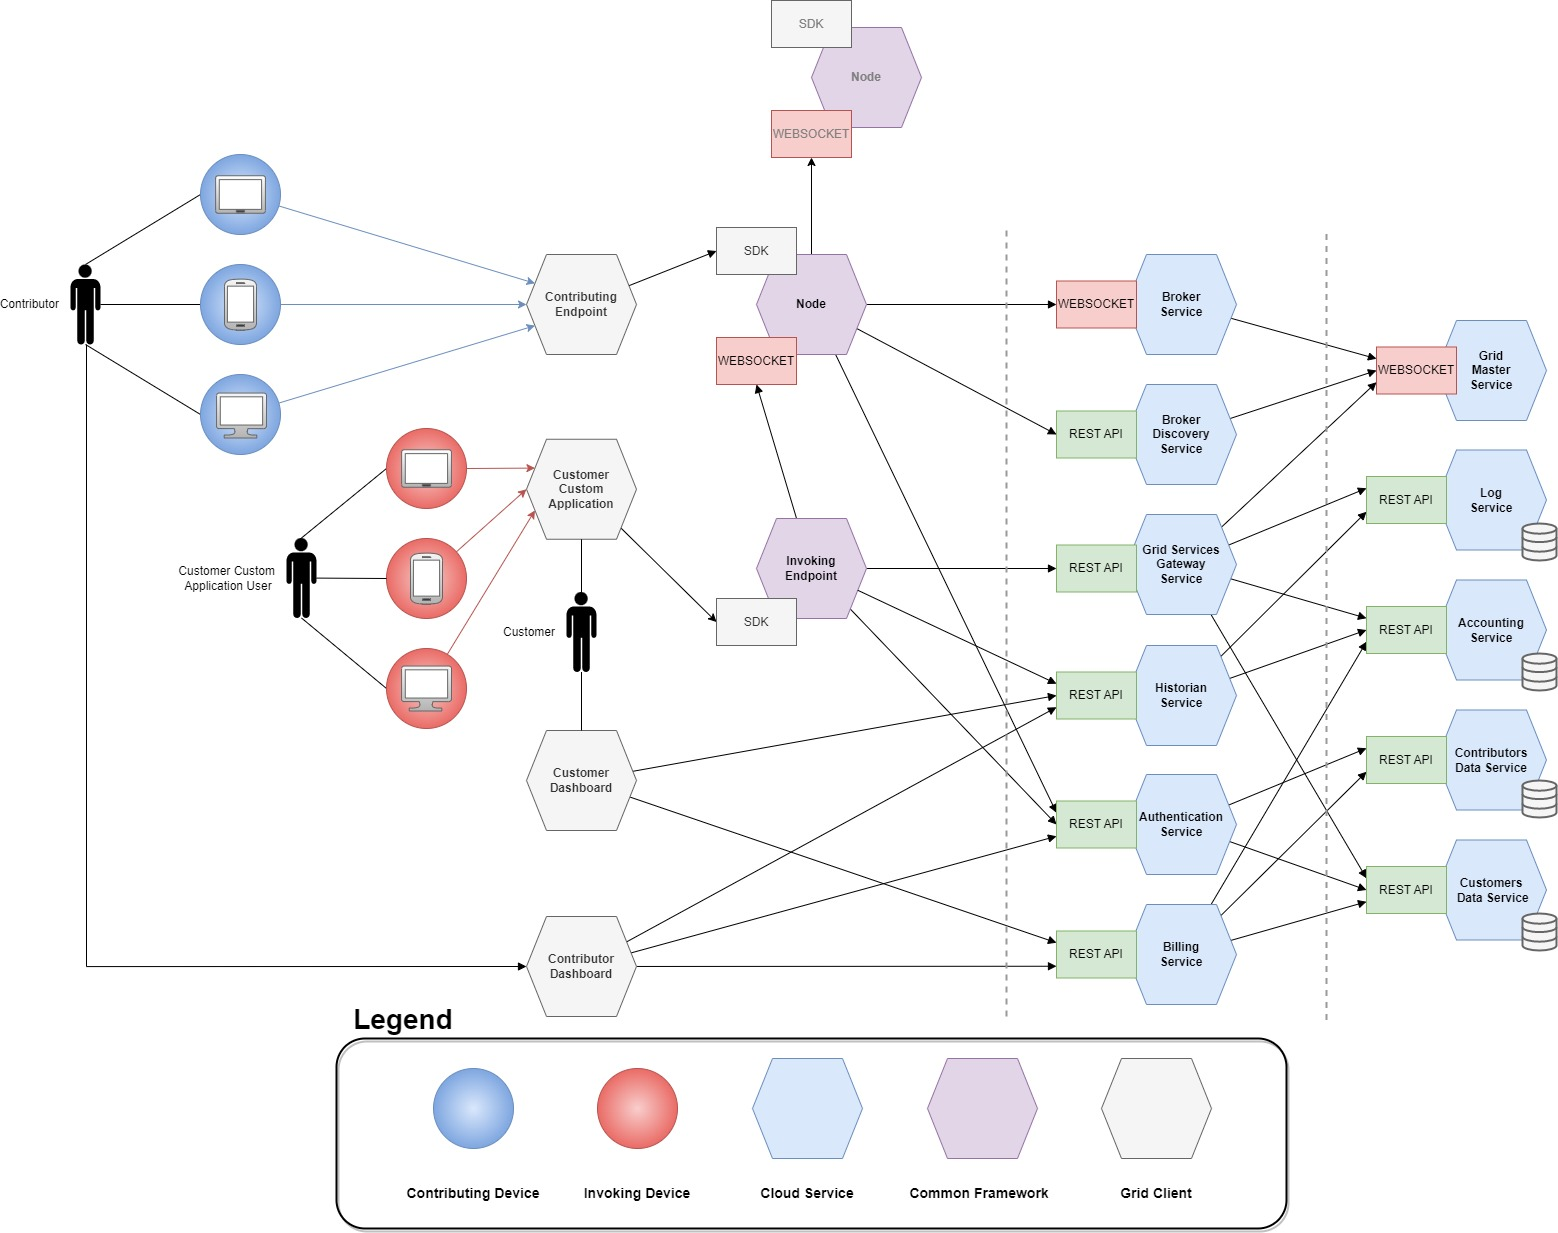
\includegraphics[width=\linewidth]{document/chapters/chapter_6/images/architecture_complete.jpg}
    \caption{Complete view of the Architecture}
    \label{fig:architecture_complete}
\end{figure}

\subsection{Cloud Services Area}\label{cloud_services_area}
The Cloud services follow a Hexagonal architecture composed by a multitude of microservices (\textit{Figure \ref{fig:architecture_cloud_services}}). Each Microservice is accessed through communication interfaces (whether Rest APIs or Web Sockets, depending on the particular microservice needs) and belong to one of the following layers:
\begin{itemize}
    \item \textbf{Business logic}\\
    Microservices that expose core business logic for Grid functionalities realization and data managing. Entities that  reside here are protected, meaning that they are isolated from the outside and their functionalities can only be accessed through the entities placed in the Adapters layer.
    \item \textbf{Adapters}\\
    Microservices that expose functionalities accessed by the entities residing in the Contributor and Customer area; such functionalities are realized through combining the services offered by entities residing in the Business logic layer.
\end{itemize}
\begin{figure}[!ht]
    \centering
    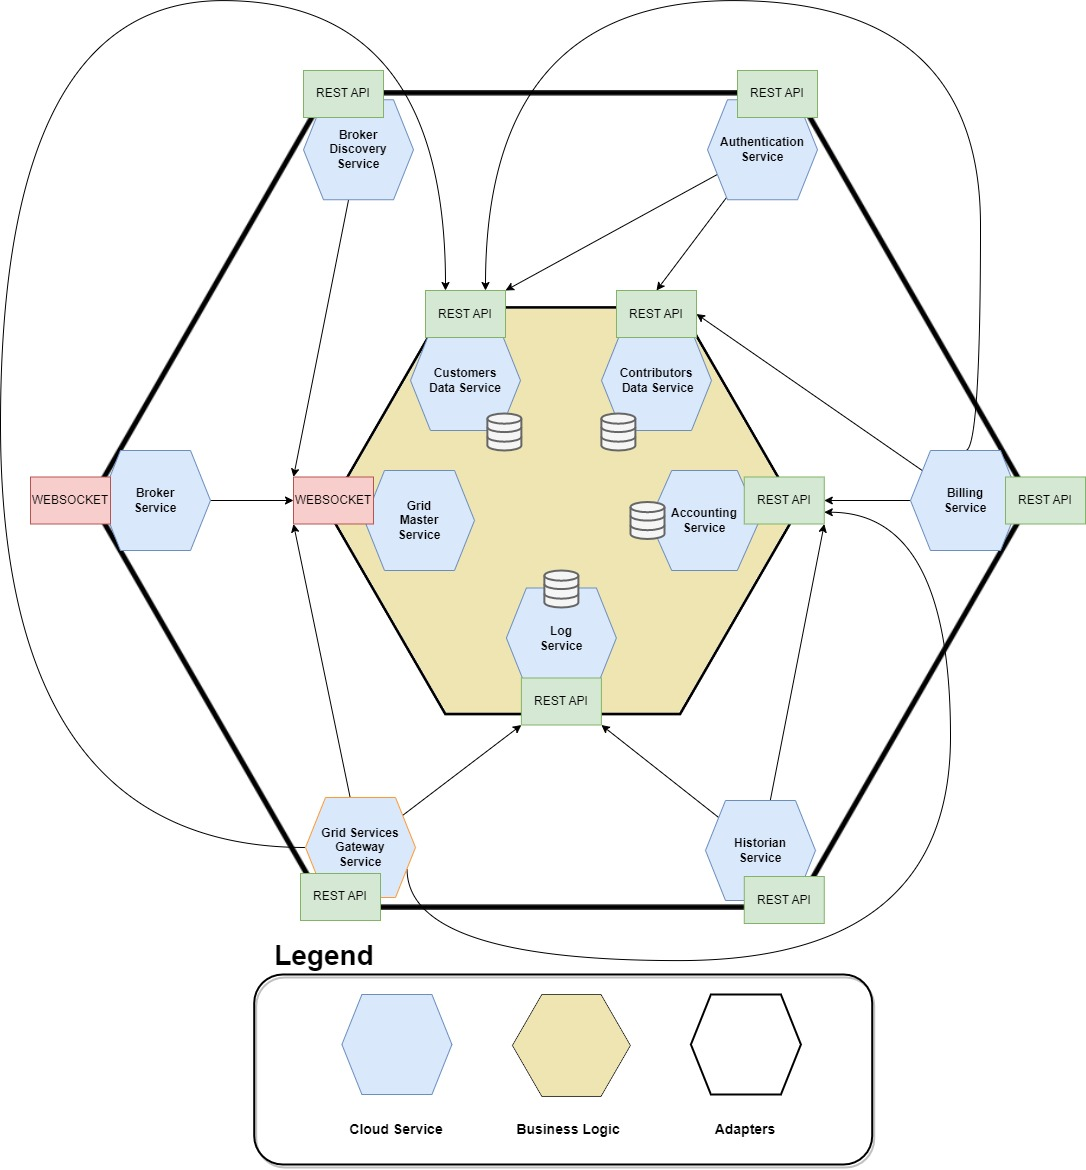
\includegraphics[width=\linewidth]{document/chapters/chapter_6/images/architecture_cloud_services.jpg}
    \caption{Architecture: Cloud Services}
    \label{fig:architecture_cloud_services}
\end{figure}

\subsubsection{Business Logic}
TODO

\subsubsection{Adapters}
TODO

\subsection{Contributor area}\label{contributor_area}
TODO

\begin{figure}[!ht]
    \centering
    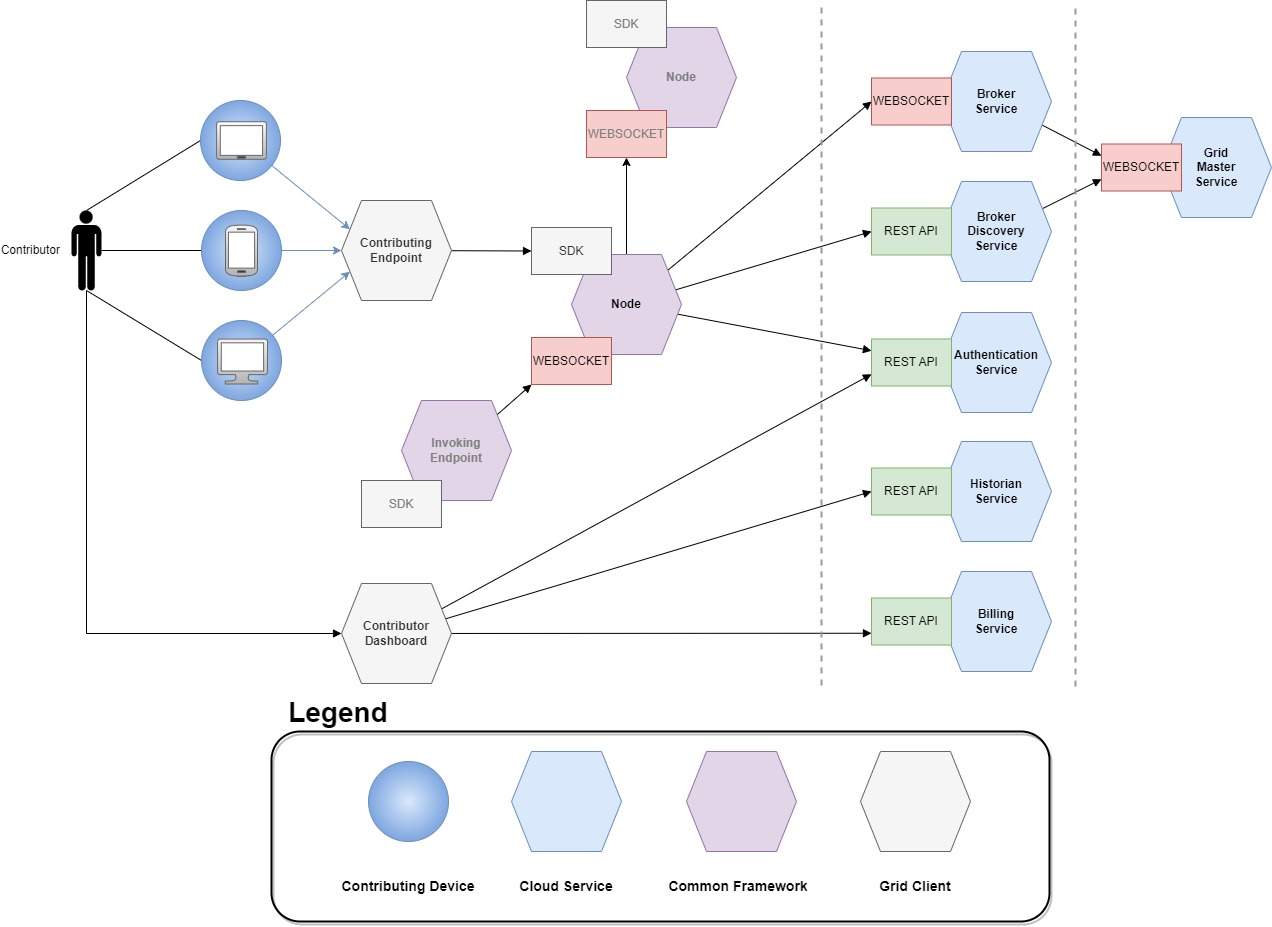
\includegraphics[width=\linewidth]{document/chapters/chapter_6/images/architecture_contributor.jpg}
    \caption{Architecture: Contributor-relevant view}
    \label{fig:architecture_contributor}
\end{figure}

\subsubsection{Node}
TODO
% High level grid draw.io: High level grid and Load Balancing

\subsubsection{Contributing Endpoint}
TODO
% Focus on interfaces and device-specific stuff

\subsubsection{Contributor Dashboard}
TODO
% Mockups

\subsection{Customer area}\label{customer_area}
TODO
\begin{figure}[!ht]
    \centering
    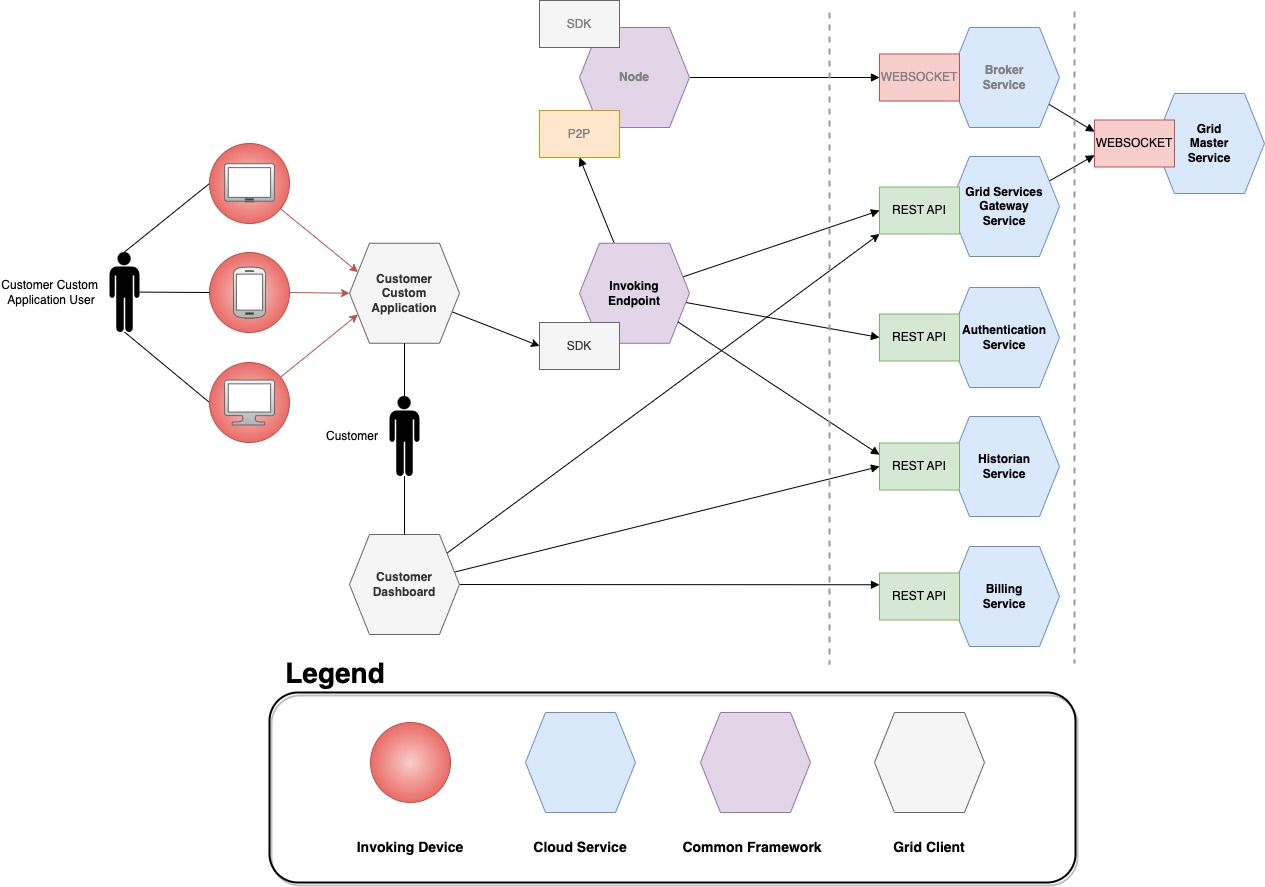
\includegraphics[width=\linewidth]{document/chapters/chapter_6/images/architecture_customer.jpg}
    \caption{Architecture: Customer-relevant view}
    \label{fig:architecture_customer}
\end{figure}

\subsubsection{Invoking Endpoint}
TODO
% High level grid draw.io: something similar to MapReduce but for a general task

\subsubsection{Customer Custom Application}
TODO
% focus on sdk

\subsubsection{Customer Dashboard}
TODO
% Mockups